\documentclass[11pt, letter]{article}
\usepackage[margin=0.7in]{geometry}
\usepackage{graphicx}
\usepackage{listings}
\lstset{
  basicstyle=\ttfamily,
  mathescape
}

\title{CS 381 - A7}
\author{Martin Mueller}
\date{Due: April $17^{th}$ 2020}

\begin{document}

\maketitle

We start by constructing a grammar for the language of $P$:
\begin{lstlisting}
    S $\rightarrow$ A | B | C
    A $\rightarrow$ {AB} | AA | $\lambda$
    B $\rightarrow$ [BC] | BB | $\lambda$
    C $\rightarrow$ (C) | CC | $\lambda$
\end{lstlisting}
This grammar enforces precedence by having different levels of symbols arranged such that it is impossible to go up a level, but it is possible to go down levels so that the correct brackets are contained within each other. This grammar also allows for starting at any level and accepts the empty string. \\
Now that we have a grammar, we can construct a PDA that recognizes it. First, we initialize the stack by pushing a dollar sign onto it. Next, we push the start symbol $S$ onto it, then nondeterministically branch out until we reach the correct combination of terminals on the stack. Once the input matches the stack, then we pop all the terminals on the stack until we hit the dollar sign. When that happens, we transition into an accept state. Notice that the PDA's stack shares the same alphabet as the grammar and the input alphabet is exactly the set of terminals in the grammar.

\begin{figure}
  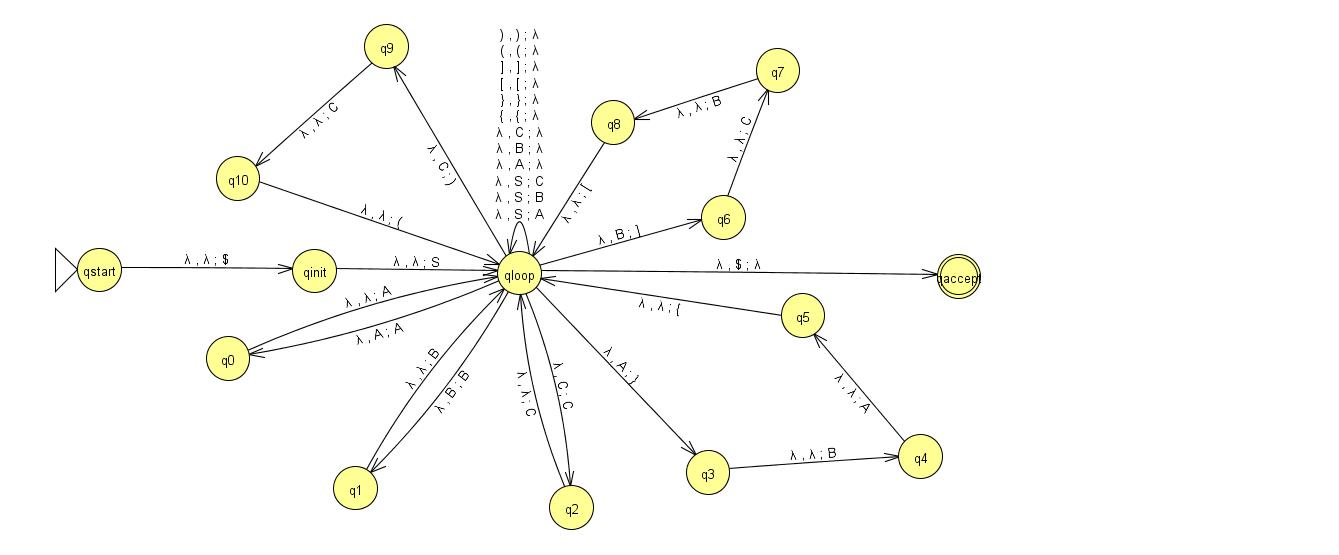
\includegraphics[width=\textwidth]{A7.jpg}
\end{figure}

\end{document}
